\documentclass[letterpaper]{article}
\usepackage[margin=1.25in]{geometry}
\usepackage{amsmath}
\usepackage{amssymb}
\usepackage{titling}
\usepackage{graphicx}
\usepackage{caption} 
\usepackage{float}
\usepackage{subfig}
\usepackage{enumitem}
\usepackage{parskip}
\usepackage{titlesec}
\usepackage{mathtools}
\usepackage{url}

\usepackage[backend=biber,style=apa,citestyle=authoryear]{biblatex}

\addbibresource{citations.bib}

\allowdisplaybreaks
\title{
	\textbf{Politech Mathematical Group} \\ 
	\vspace{2ex} 
	Political Fatness Report
	\vspace{2ex}
}
\author{
	Darren Kong \\ 110770716
	\and 
	Hugo Mainguy \\ 111747982
	\and 
	Jeffrey Zhong \\ 112299792
	\vspace{3ex}
}
\date{March 8, 2021}

\begin{document}


\begin{titlepage}
\maketitle
\thispagestyle{empty}
\end{titlepage}

\section{Abstract}
%TODO%
%needs to be written (let’s aim for maybe 150 words max? Is that how people do this here?)%
The issue of gerrymandering has long been an issue in the United States, as many criteria are considered in the process of creating fair districting plans, and these criteria differ from state to state. Some cases in the past have used the Polsby-Popper test as one way to calculate compactness as a measure of gerrymandering, and the test generally favors geometrically compact shapes. However, Polsby-Popper does not account for the distribution of the population within the shape, and as such, may unnecessarily punish non-compact districtings. The paper therefore investigates an alternate compactness measure that factors in the distribution of the population alongside the geometry of a districting: Population atness. Using the ARS, we calculated the population fatness alongside the Polsby-Popper score for the districts of several U.S. states. Graphing the results, we examined the extrema in each quadrant to determine the attributes that most affect each measure. It may be of interest to weigh the Polsby-Popper test score and the population fatness score together for a better measure of compactness. 


\section{Introduction}

The advent of technology, especially in more recent times, has made every aspect of life “more” something. For instance, we are more connected with the Internet and instant communication across the globe than we were with letters, or printed newspapers. It may seem that this intensification of long-distance communication should make us all closer to one another. Yet, it seems that technology has also made mankind more divided, with the decentralization of news outlets or American politics. With the advent of technology, the decennial process of redistricting states with more than one congressional district has become a partisan affair. Fewer districts are competitive now than even twenty years ago such that there is less need to appeal to the other side (\cite{cook}). Artificial intelligence applied to redistricting has contributed to a polarization of American politics; however, if used with good intentions, it could become the very solution to a problem that it fueled in the first place.

It is easy to call out gerrymandering, yet, at the same time, difficult to give precise measures for it. In Vieth v. Jubelirer, ruled in 2004, the Supreme Court argued that a districting was not gerrymandered for there was no measure to quantify inequality or lack of fairness. (\cite{vieth}) As courts – especially the Supreme Court – often rule by precedent, this has been used as an excuse to bring down some cases that made it to the highest court of the land. This has emboldened strategists to make increasingly “unfair” maps. The surge in gerrymandered districting plans is the combination of three factors that all came together at the same time: large political successes for one party, the Republicans, just before drawing districts, the sudden improvement of technology, and the increasing polarization in voting patterns.

%Needs some sources for the claims here%

This comes together in what could be considered a paradox: while there are ever more accurate methods to gerrymander at will, there is no mathematical standard accepted by the courts to identify the practice as of today. Furthermore, state constitutions tend to lag even further behind, because of the amount of the slow legislative process and support required to change them. Only twenty-three states require their congressional districts to be contiguous. (\cite{contiguity}) While in practice, this is virtually always the case, it creates more potential for gerrymandering in over half of the states. (Contiguity refers to the fact that any point of the district must be accessible from any other point of the district without leaving it, except for example if part of it is an island and there is a method of transportation such as a bridge or a regular ferry between both sides.) Furthermore, only eighteen states have any mention of compactness for their congressional districts. Within those eighteen states, a minority have more requirements. For instance, Iowa requests that districts not be oddly shaped (the state is almost a rectangle that can be split equally in four rectangles), California asks for districts not to bypass nearby large population areas for more distant populated areas, Arizona requires at least some of the districts to be competitive if feasible, and Rhode Island to represent the state fairly (although it currently has two congressional districts and will most likely lose one after the 2020 Census reapportionment.) (\cite{contiguity}) Overall, there is a lot of leeway in what can be done by the redistricting committee. 


\section{Methodology}
To counter this, we suggest setting a standard with a definition of compactness. Compactness is something easily perceivable by humans, yet, there is no measure that satisfies human perception all the time - and we sometimes disagree among ourselves, as shown by Kaufman et al. (\cite{king})
However, a generally sensible choice is using the Polsby-Popper measure, which is given by the formula:

\[
	PP(D) = \frac{4\pi A(D)}{P(D)^2}
\]

% Need sources for these claims

Where A(D) is the area of the object D and P(D) its perimeter. This gives us a ratio between 0 and 1. It is 0 precisely when the area is 0 (D is a line or a point) and 1 when D is a circle. In particular, this favors compact round objects, and defavors those with longer or jagged perimeters. Both of these are important, and the measure has been used in real life, for instance with Arizona’s redistricting in 2000. (\cite{moncrief})It is noteworthy that several states use different measures, particularly in the West, where more attention is paid to fairness.
% Citation needed%
Other measures are used in different states: for instance, in Colorado, the districts should minimize the total perimeter. States like California and Michigan instead focus on dispersion rather than contorted boundaries, as Moncrief points out. 

It becomes evidently clear that the Polsby-Popper measure only takes into consideration the geometric compactness or fatness of the redistricting shape. A more suitable measure for compactness would also take into consideration the population requirement of the districtings. All congressional districtings have to be equal in population at the time of the redistricting. For example, a congressional district may seem to be shaped oddly but that is only due to the legal requirement for equal population size.

Simultaneously, it became clearer that while a non compact district is almost always subject to gerrymandering, the converse is not always true. One example of this is when districts bypass population centers nearby to instead include populations that are further away.
Here we will propose an alternative to the Polsby-Popper that will be referred to as the Population Fatness measure, or Fatness for brevity. 
To calculate this measure, we used the following formula:

\[
	\frac{POP(\text{D})}{POP(\text{BC(D)})}
\]

Where D represents the district D, CH(D) is the convex hull that contains D, and POP(D) is the population in D. This measure utilizes precincts as the base level of a population cluster. Since the bounding circle cuts through some precincts, in those cases, the ratio of the area of the precinct in the convexhull is used to estimate the population of the part of the precinct inside of the bounding circle, yielding good approximations. Since precincts form districts, we do not need to apply any ratio other than 1 for the population inside the district borders. Furthermore, this measure only takes into account the population that is inside the state, as the population outside of the state but inside the convex hull should not influence the districts. Once again, a perfect score of 1 comes when the district geometry itself is a convex hull, and a low score close to 0 comes when the convex hull encompasses many populous precincts, large areas of land, or a combination of both outside of the district's borders.

%[We should probably include the code for the two measures here, if anyone feels like adding it. Actually, maybe after each measure, whatever is better.]%

Since these two measures are different, it is interesting to compare them to see when they are similar and when they differ, explain why that is the case, and conclude whether those districts are gerrymandered or not. Using the current congressional districts, here are the data points found (Pennsylvania and North Carolina maps are from 2016).

\section{Results}

\begin{figure}[H]
	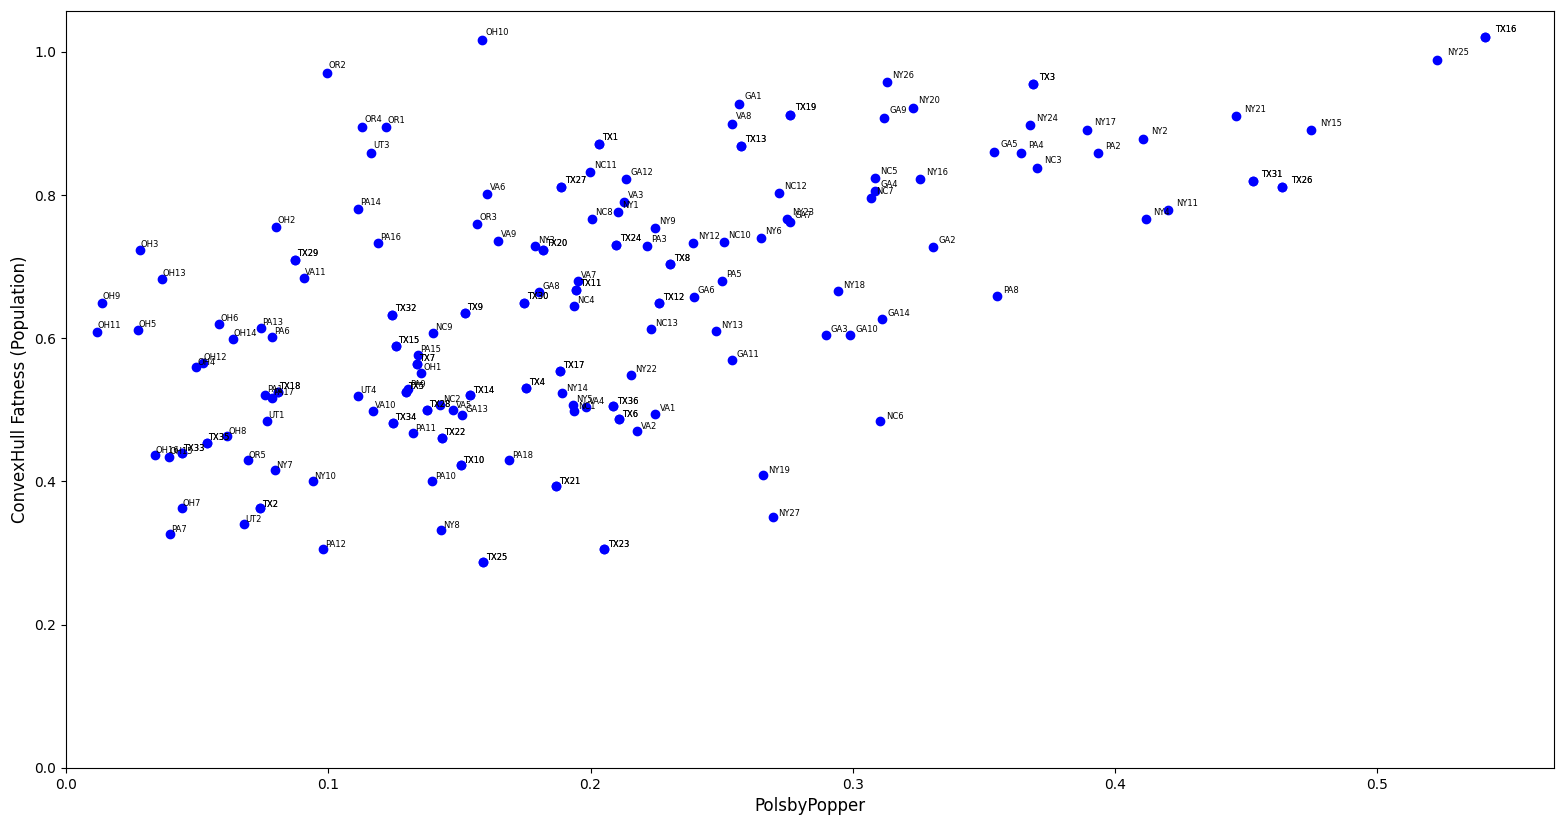
\includegraphics[width=\linewidth]{./figures/convexHullPopulationFatnessVPP.png}
	\caption{Plot of Population Fatness v. PolsbyPopper}
	\label{fig:datapoints}
\end{figure}

%We need a better name for this section
\section{Research}
From the results, we can see compare each district's Fatness score with its Polsby-Popper score. To help easily identify specific districts, we will split the graph into four quadrants. The quadrants are to be referred from 1 to 4 starting from the top right in a counterclockwise fashion. We do this to identify extremeties in each of the district scores to see in what cases these two scores may differ wildly.

\begin{figure}[H]
	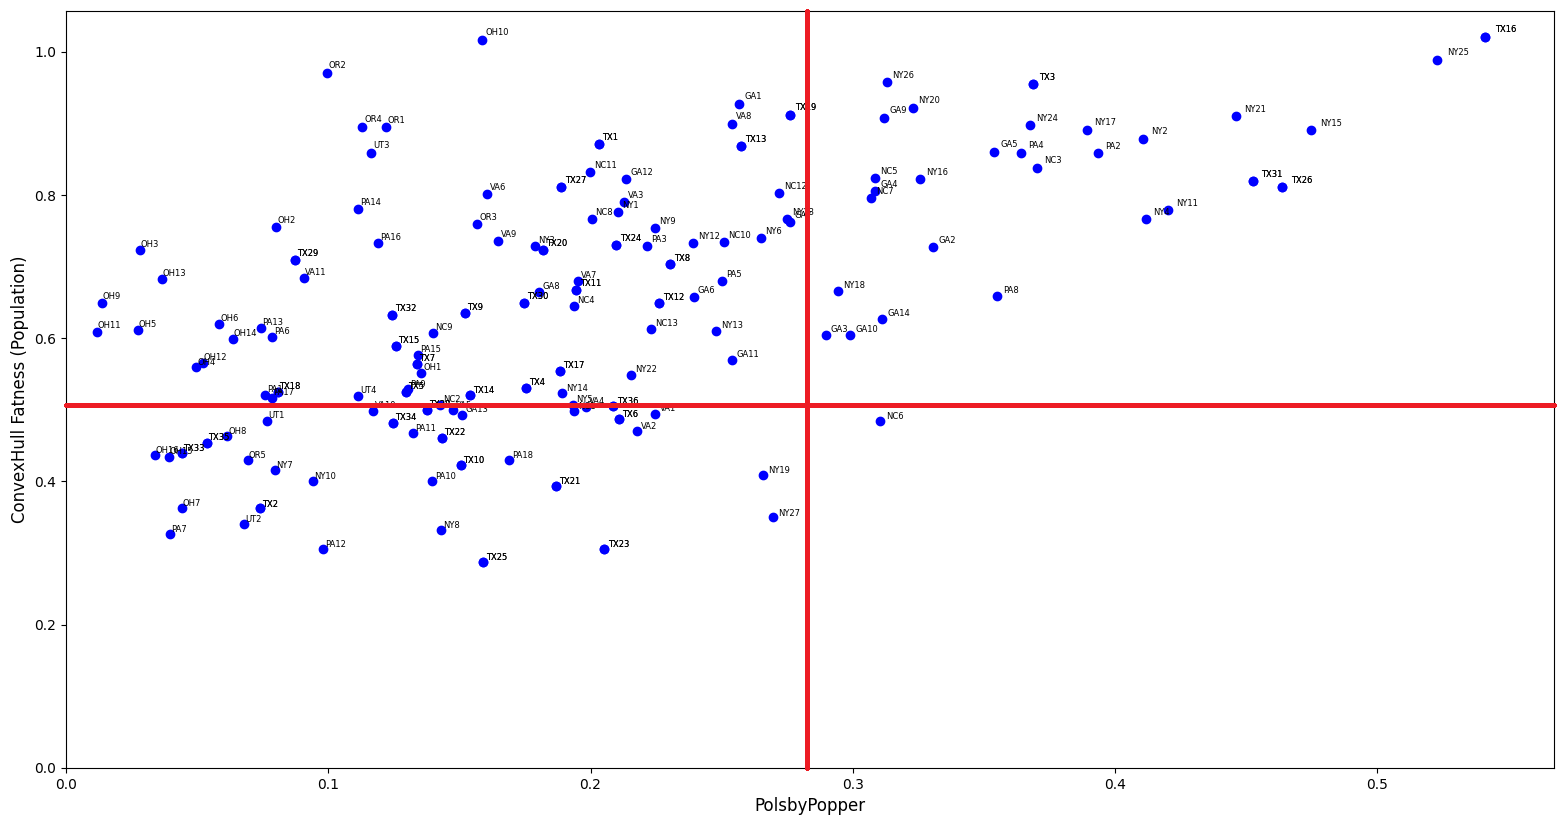
\includegraphics[width=\linewidth]{./figures/convexHullPopulationFatnessVPPQuadrants.png}
	\caption{Plot of Population Fatness v. PolsbyPopper Edited}
	\label{fig:datapointsEdited}
\end{figure}

\subsection{Low Fatness and High Polsby Popper}
We will make a quick remark on the fourth quadrant. This is the quadrant where we would have a low Fatness score and a high Polsby Popper score. The point of this quadrant is to find the districts which Polsby Popper identifies as a good district but Fatness identifies as a bad district. In essence, if we use Polsby Popper to categorize good and bad districts, this quadrant would represent the False Positive. It is mostly empty except for the inclusion of North Carolina's 6th congressional district.
%Insert NC-06
This district is actually near average on the Fatness score and PolsbyPopper score. It does seem to be an average district since it leaves the square shape near Greensboro to include the city of Winston Salem. The extrusion into Winston Salem seems to be jarring due to the initial square shape.

\subsection{High Fatness and High Polsby Popper}
We will begin our look on the first quadrant, specifically NY-25, NY-15, and TX-16. The district scores for both the Fatness and Polsby-Popper measures are both high for these districts. It is rather easy to tell why.

\begin{figure}[H]
	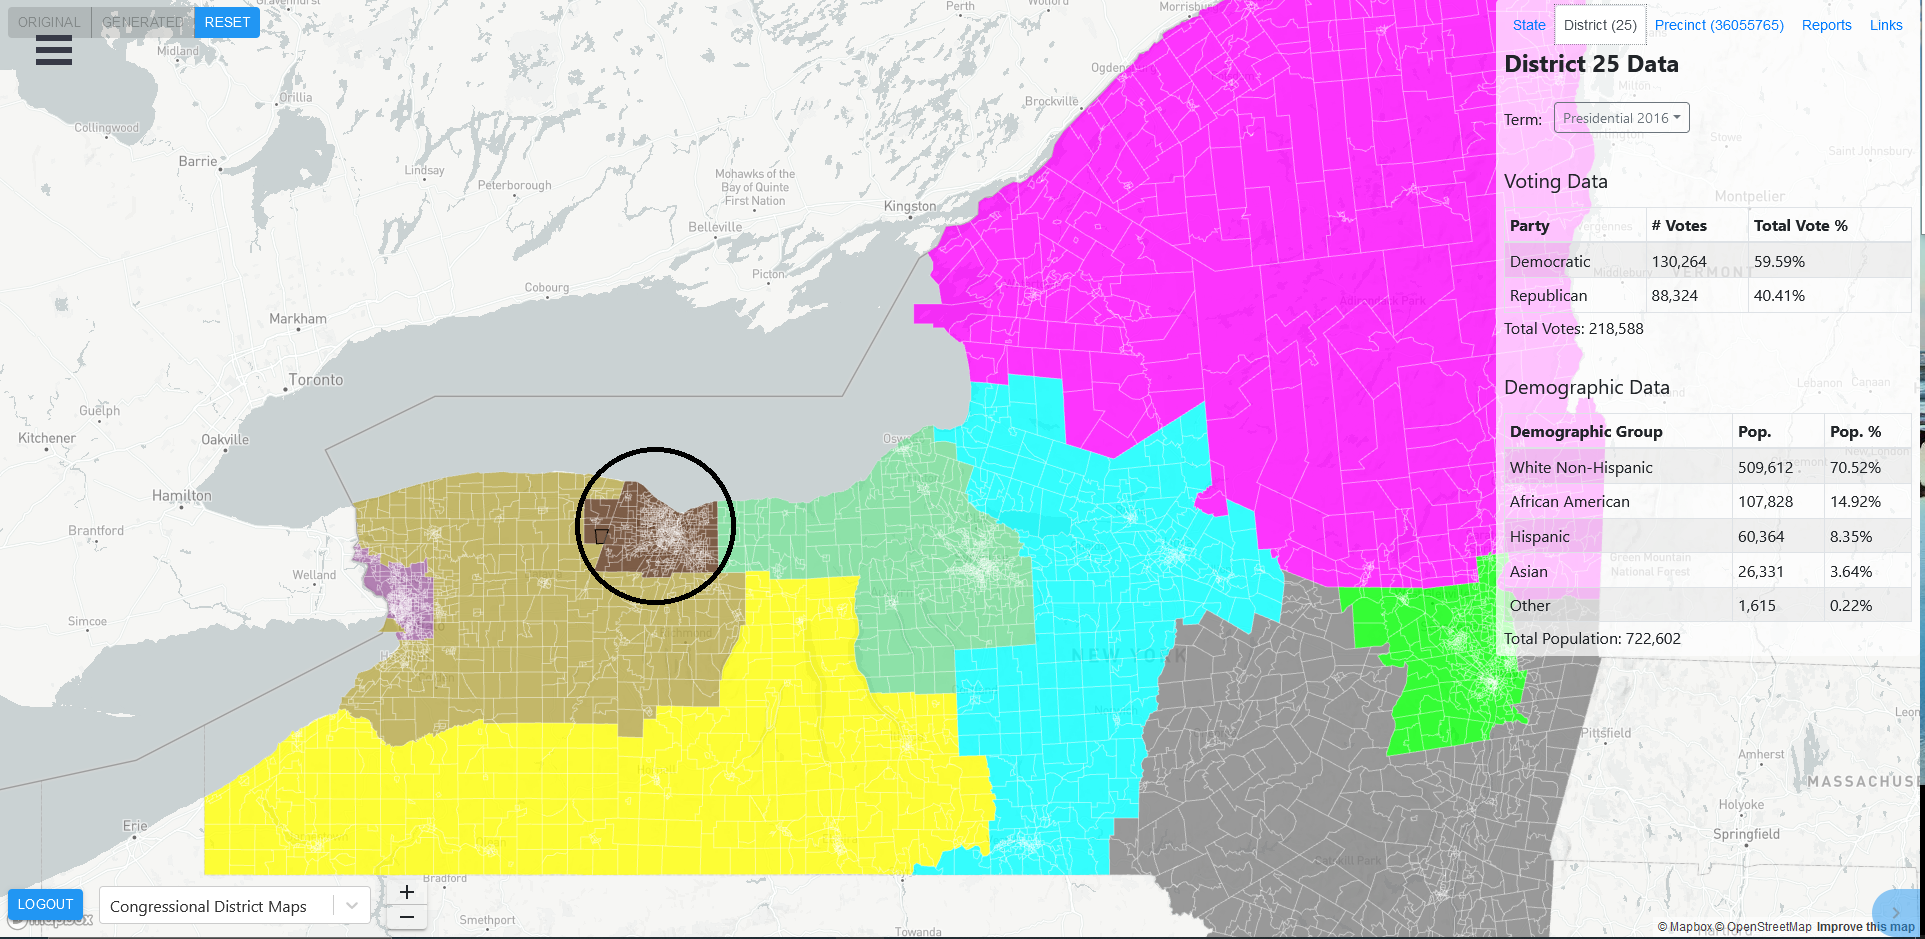
\includegraphics[width=\linewidth]{./figures/NY-25-BoundingCircle.png}
	\caption{NY-25 Bounding Circle}
	\label{fig:ny25boundingCircle}
\end{figure}

\begin{figure}[H]
	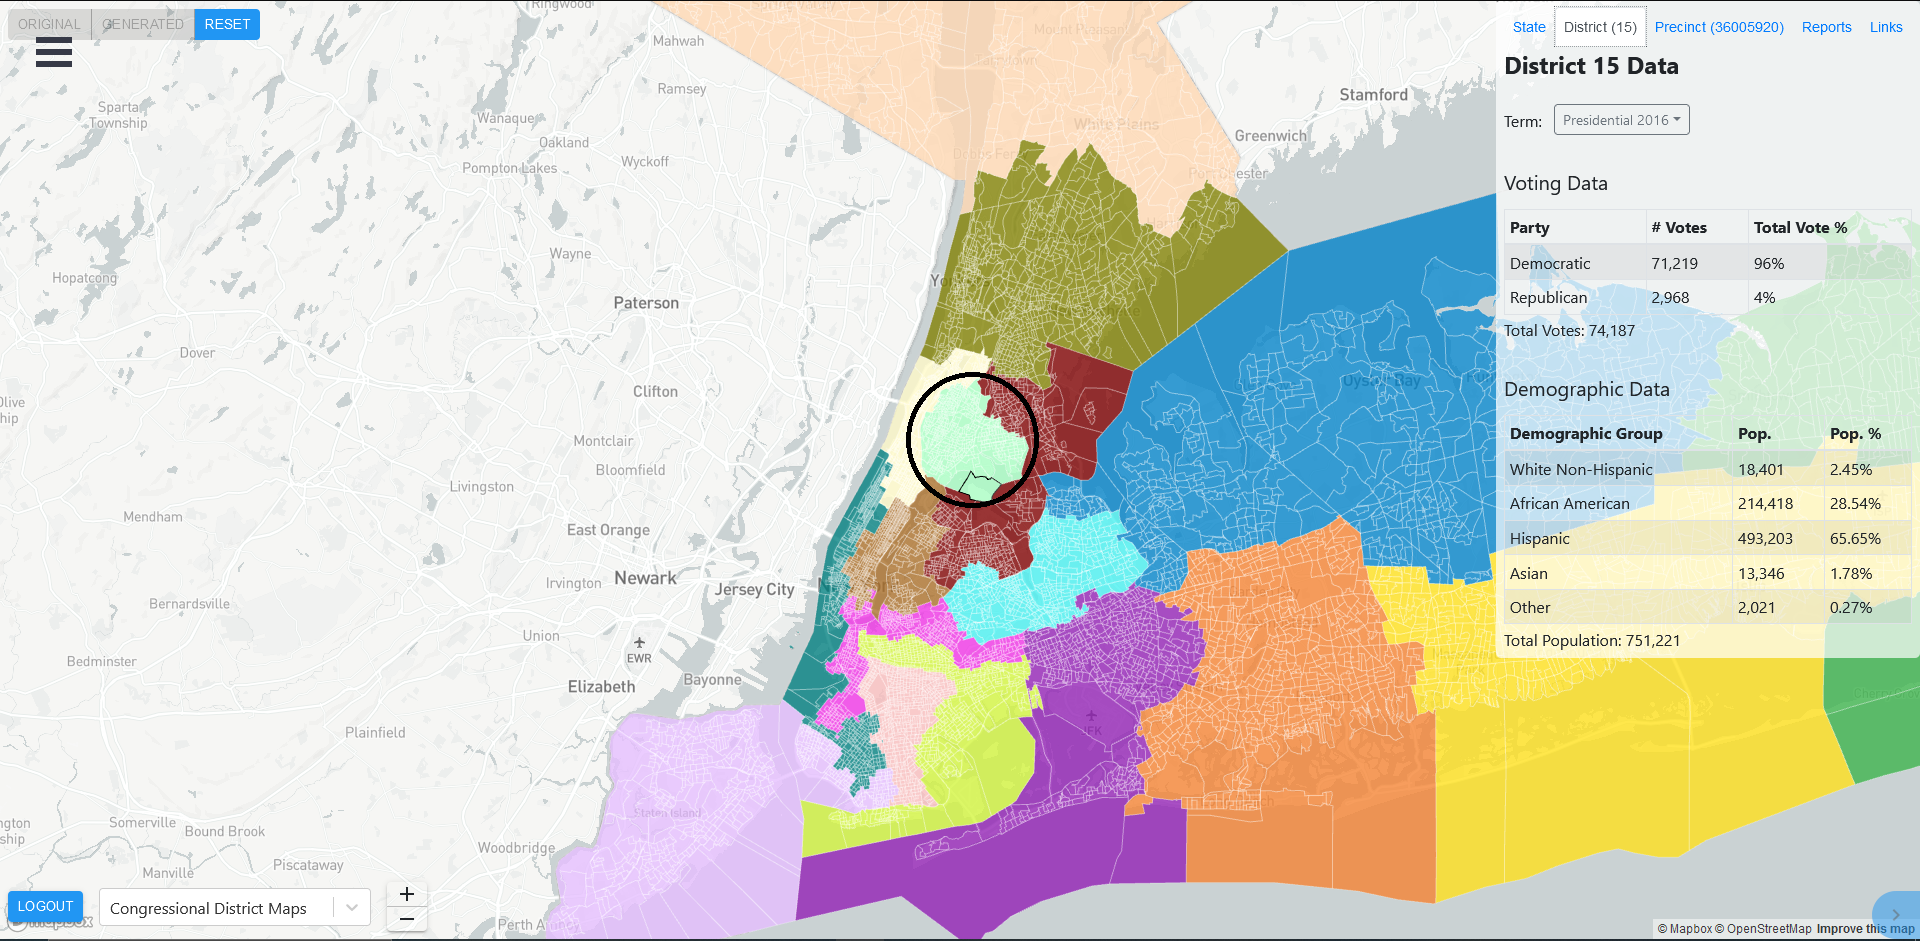
\includegraphics[width=\linewidth]{./figures/NY-15-BoundingCircle.png}
	\caption{NY-15 Bounding Circle}
	\label{fig:ny15boundingCircle}
\end{figure}

\begin{figure}[H]
	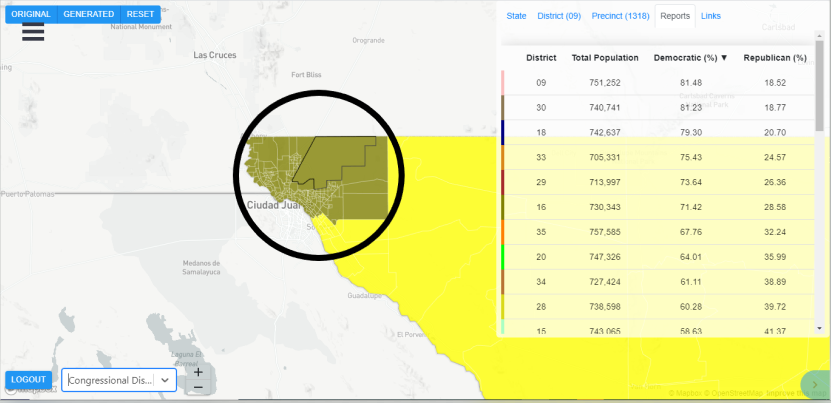
\includegraphics[width=\linewidth]{./figures/TX-16-BoundingCircle.png}
	\caption{TX-16 Bounding Circle}
	\label{fig:tx16boundingCircle}
\end{figure}

These districts are all centered around a major population hub. NY-25 is centered on Rochester, NY-15 is centered on the Bronx, and TX-16 is centered on El Paso. These districts geometrically all look compact and we believe that no one would considered them abnormal in any sense. This explains the high Polsby-Popper score and also partially explains the high Fatness score. 

Specifically for the example of TX-16 which takes advantage of being small and densely populated with sparsely populated districts and state/country borders around, along with straight, perpendicular borders for most of its contour. It is a very Democratic area surrounded by moderately Republican areas, but it forms a coherent district encompassing one city and its direct surroundings, and contains all but the southernmost part of El Paso County, making it a very reasonable district. It is a similar story for the other districts.

\begin{figure}[H]
	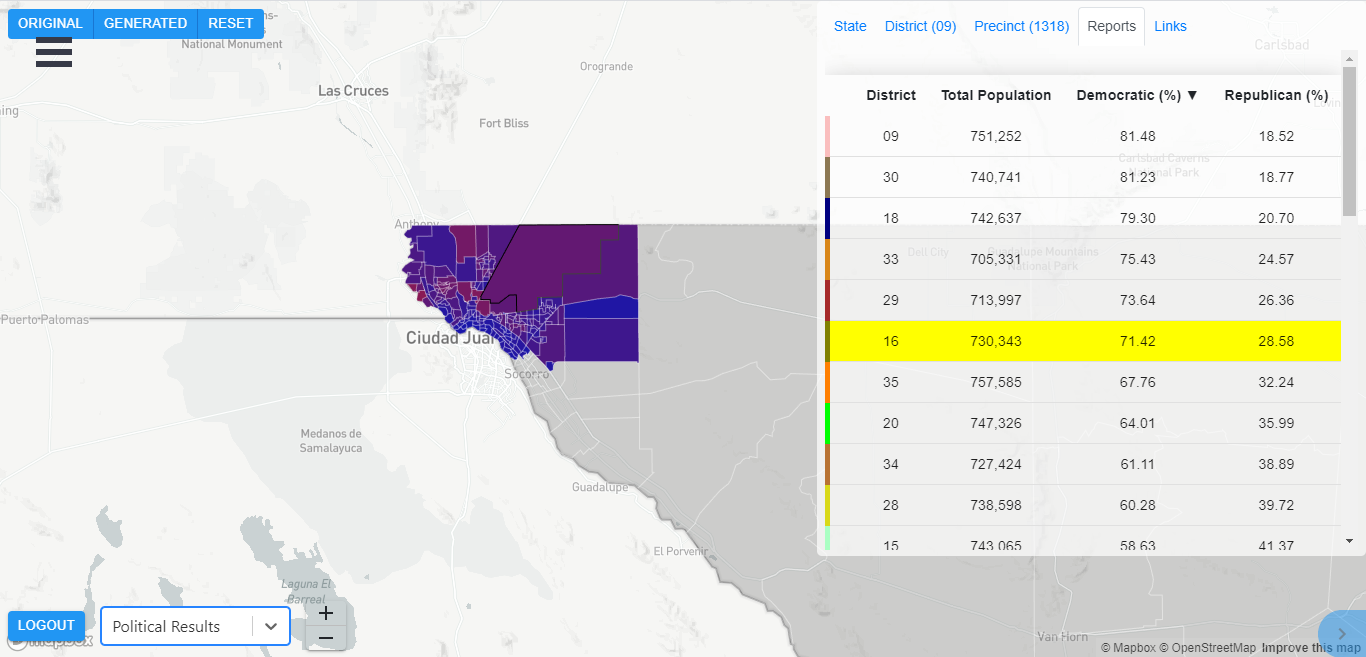
\includegraphics[width=\linewidth]{./figures/TX-16.png}
	\caption{TX-16}
	\label{fig:tx16border}
\end{figure}

\begin{figure}[H]
	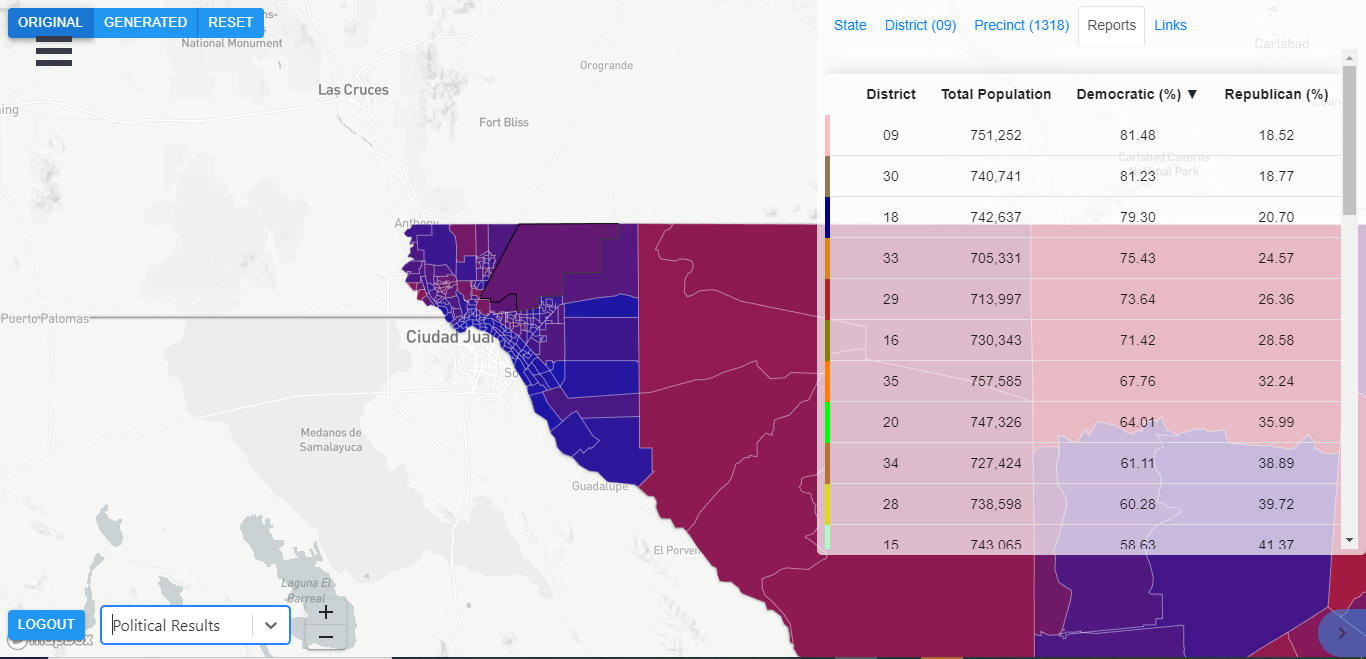
\includegraphics[width=\linewidth]{./figures/TX-16-SurroundingArea.png}
	\caption{TX-16 Political Results}
	\label{fig:tx16political}
\end{figure}

\subsection{Low Fatness and Low Polsby Popper}
We can now skip ahead to the third quadrant. These are the districts often pointed out by opponents of gerrymandering as being “bad”, failing most standard measures for compactness.


\subsection{High Fatness and Low Polsby Popper}
We now move onto the extremeties in the second quadrant. The focus will be on OR-02 and OH-10 as these two districts had the highest fatness score.

\begin{figure}[H]
	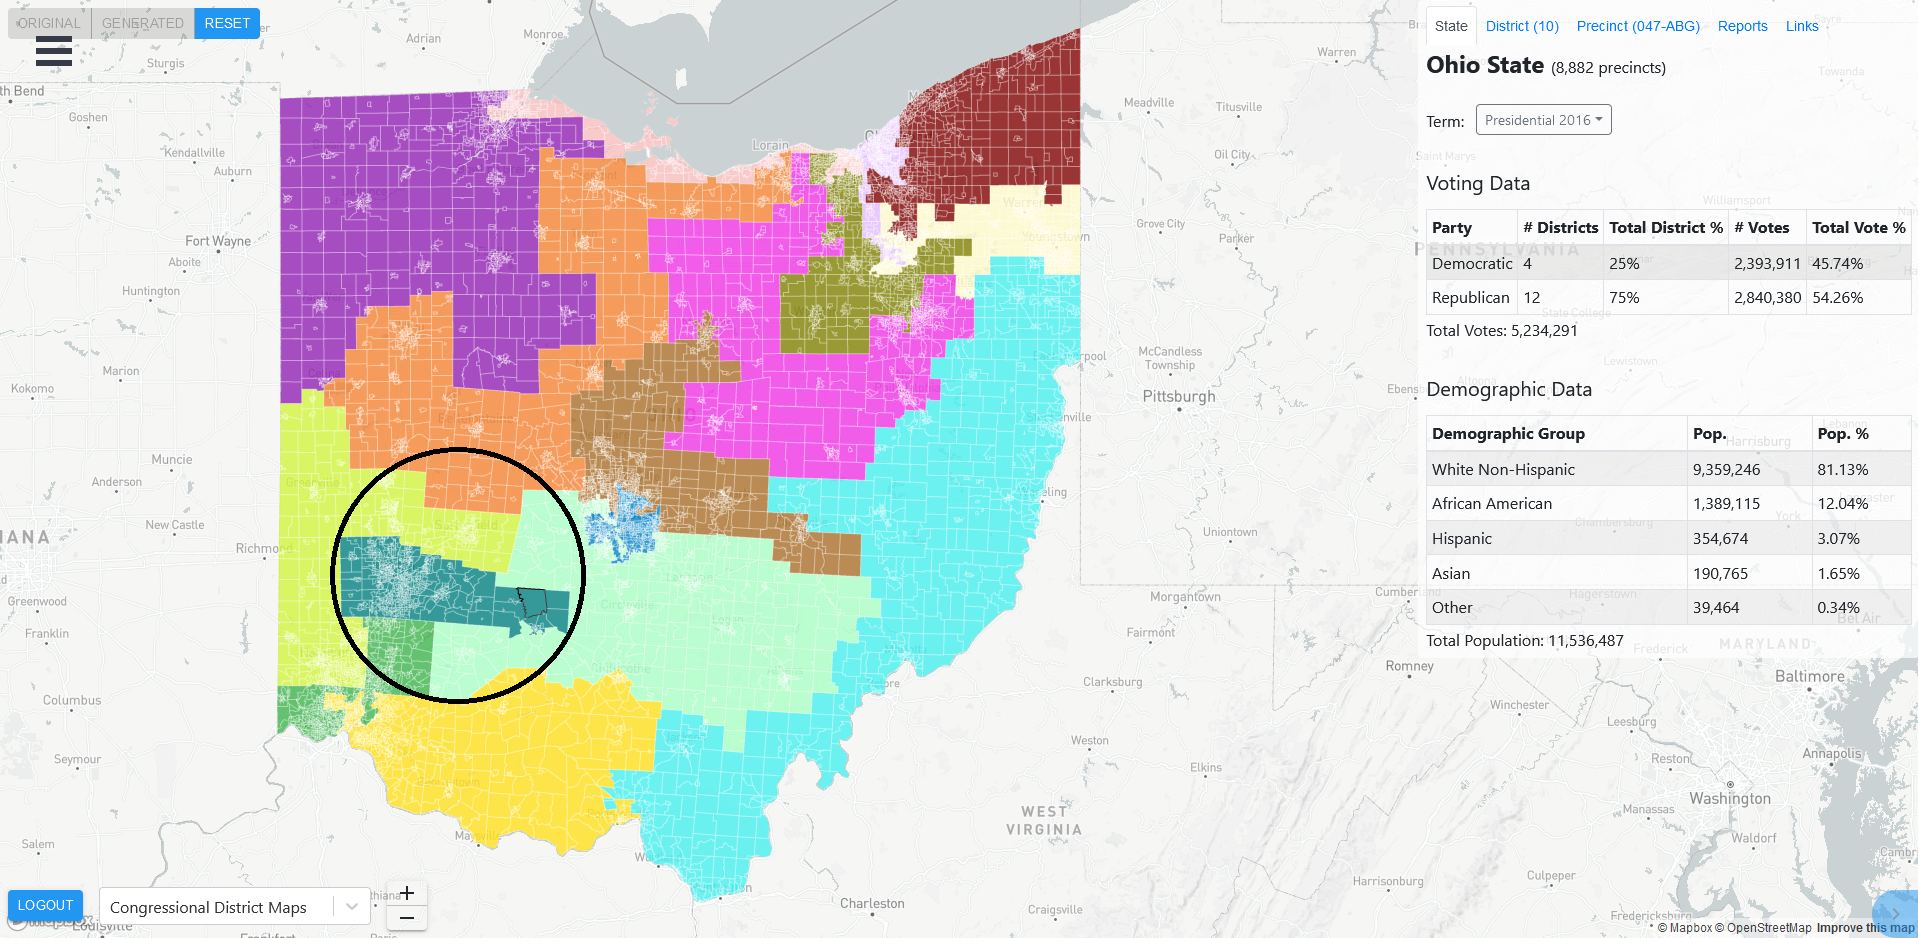
\includegraphics[width=\linewidth]{./figures/OH-10-BoundingCircle.png}
	\caption{OH-10 Bounding Circle}
	\label{fig:oh10boundingCircle}
\end{figure}

For OH-10, the Polsby-Popper measure rated this district rather low due to its long rectangle shape. Obviously, with the convex hull fatness, the score is higher as the only major difference is the removal the staircase shaped northern border of the district. Looking at the district geometrically, by itself, it would be hard to justify malicious intent.

\begin{figure}[H]
	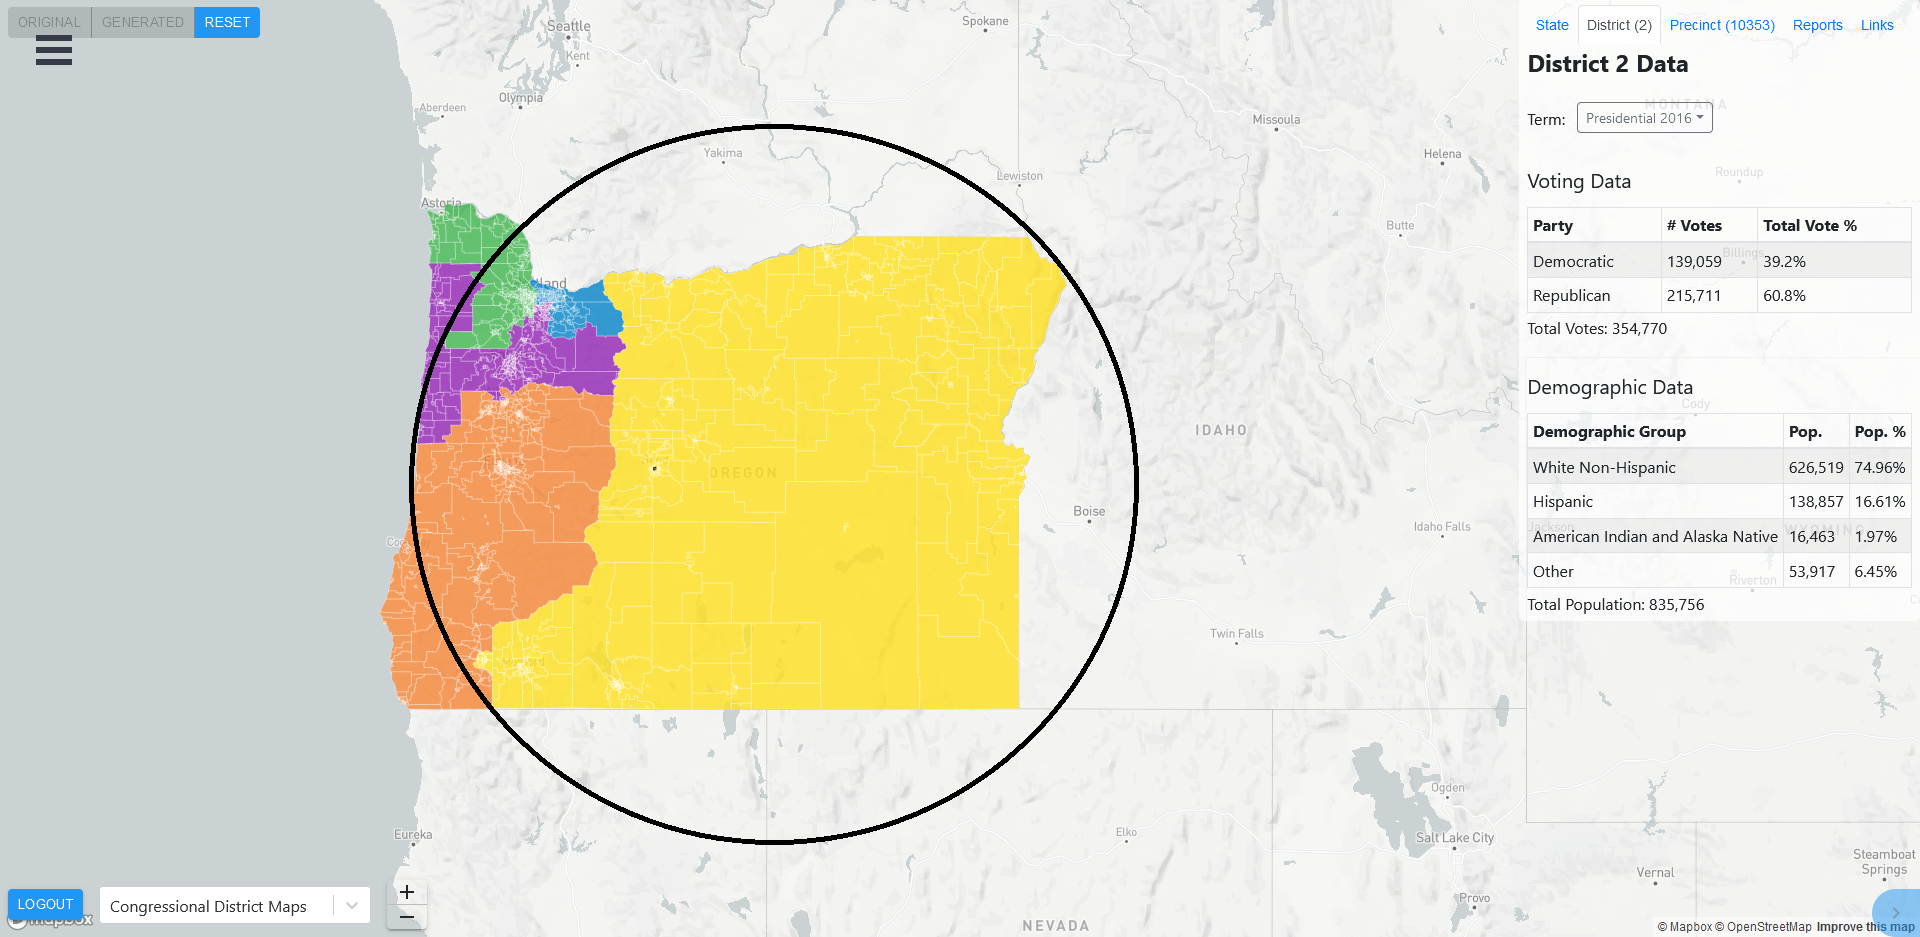
\includegraphics[width=\linewidth]{./figures/OR-02-BoundingCircle.png}
	\caption{OR-02 Bounding Circle}
	\label{fig:or02boundingCircle}
\end{figure}

A similar case can be made for OR-02. Its Polsby-Popper score was low, landing it in the left half the plot. However, it is also situated comfortable in the second quadrant where the Fatness score is high. We believe that this is a more accurate measure of the compactness of this district. There are some theories to explain the low Polsby-Popper score. If one looks closely at the border of the district, specifically the western and northern half, it is made up of jagged edges. The jagged edges constitute the district following a border represented by rivers to the north and northeast. The western portion is simply following the precincts that have the jagged edges. The many jagged edges increase the perimeter portion of the Polsby-Popper measure, therby resulting in a low score for this district. The convex hull measure is not effected as much by the jagged edges as it would change little in terms of the population that is included. Furthermore, the jagged edges are borders to the Willamette National Forest which would obviously be have a low population density even if it is included.

Similar reasonings can be made for OR-04 and OR-01. Even though OR-01 seems to have a "Pac-Man" shape, the convex hull simply adds the Tillamook State Forest.
%\begin{figure}[H]
%	\includegraphics[width=\linewidth]{./figures/OR-04.png}
%	\caption{Oregon District 06}
%	\label{fig:or04border}
%\end{figure}

%\begin{figure}[H]
%	\includegraphics[width=\linewidth]{./figures/OR-01.png}
%	\caption{Oregon District 01}
%	\label{fig:or04border}
%\end{figure}

The Convex Hull Fatness is not without its own faults. For example, OH-06 has scored much higher than in the Circle Fatness measure. An explaination of why it was considered a bad district was elaborated on previously. However, due to the new measure of fatness, it follows the same reasoning as OH-10. The difference here is that OH-10 does not seem to avoid any major population centers. However, an arguement can be made that OH-06 avoids the Democratic leaning city of Athens. It is not the most egregious district in terms of compactness but it seems to be elongated with intent. A better example of this comes with TX-15 and TX-34 which both have similar reasonings as OH-06.

\begin{figure}[H]
	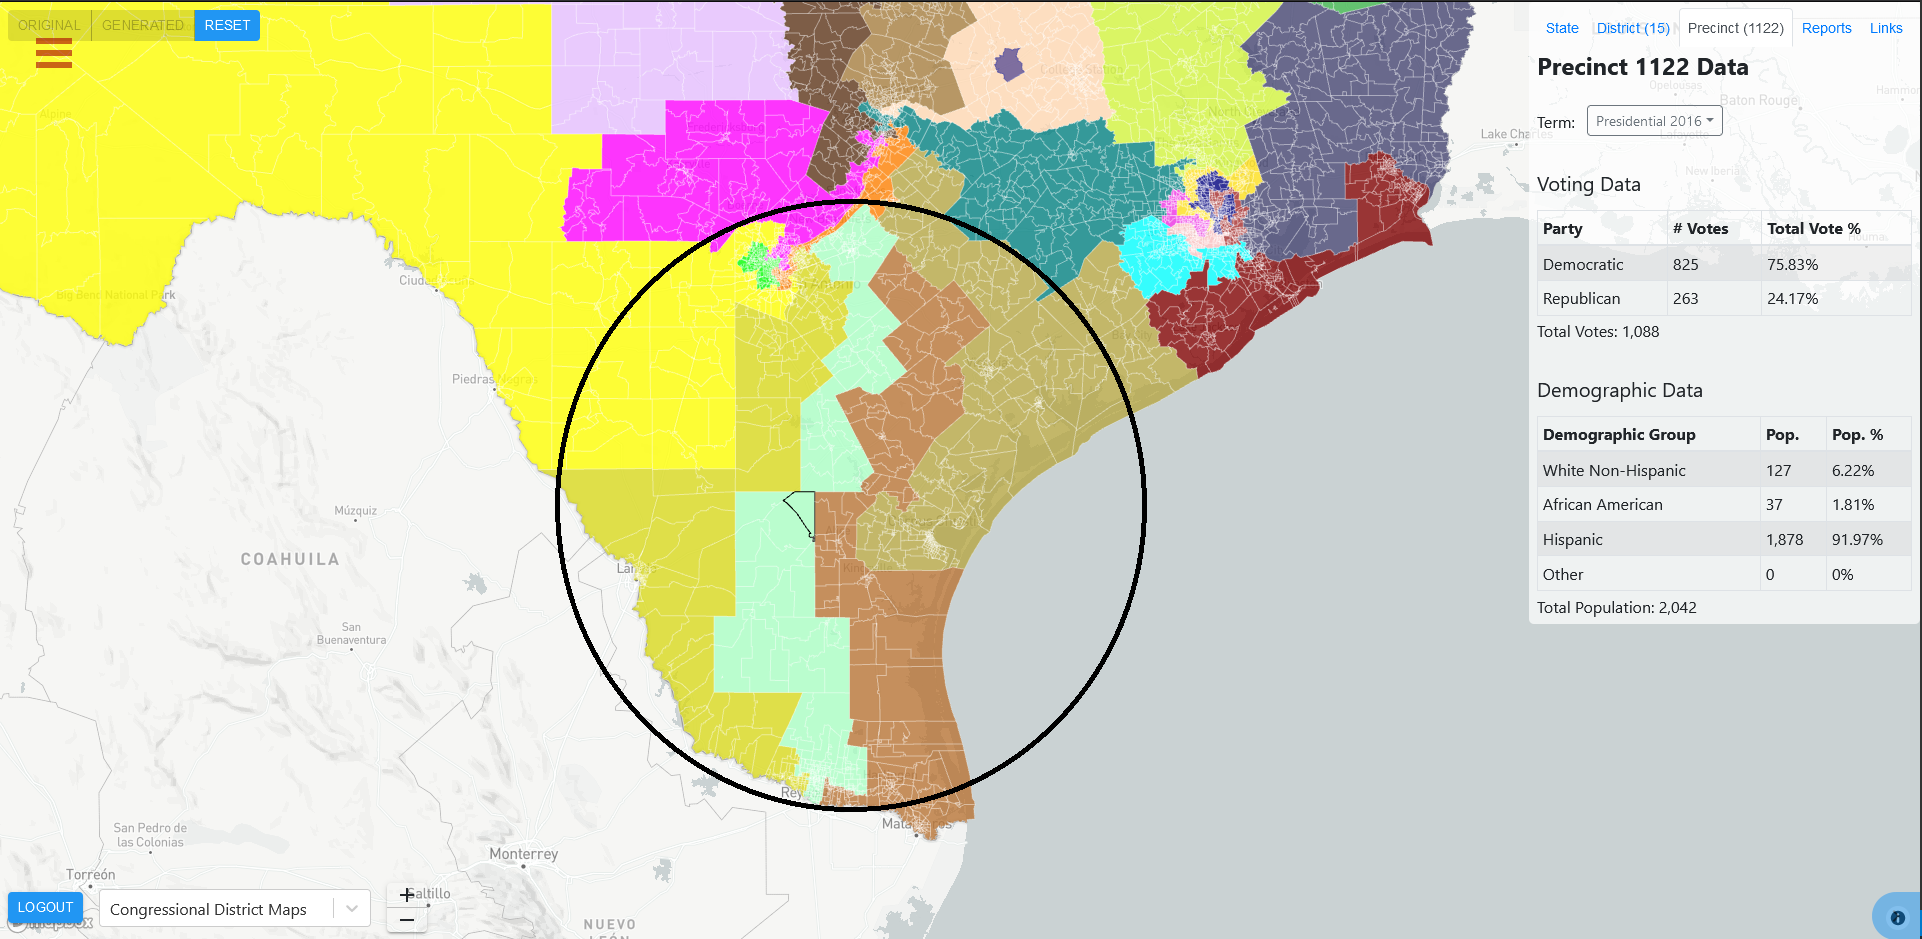
\includegraphics[width=\linewidth]{./figures/TX-15-BoundingCircle.png}
	\caption{TX-15 Bounding Circle}
	\label{fig:tx15boundingCircle}
\end{figure}

\begin{figure}[H]
	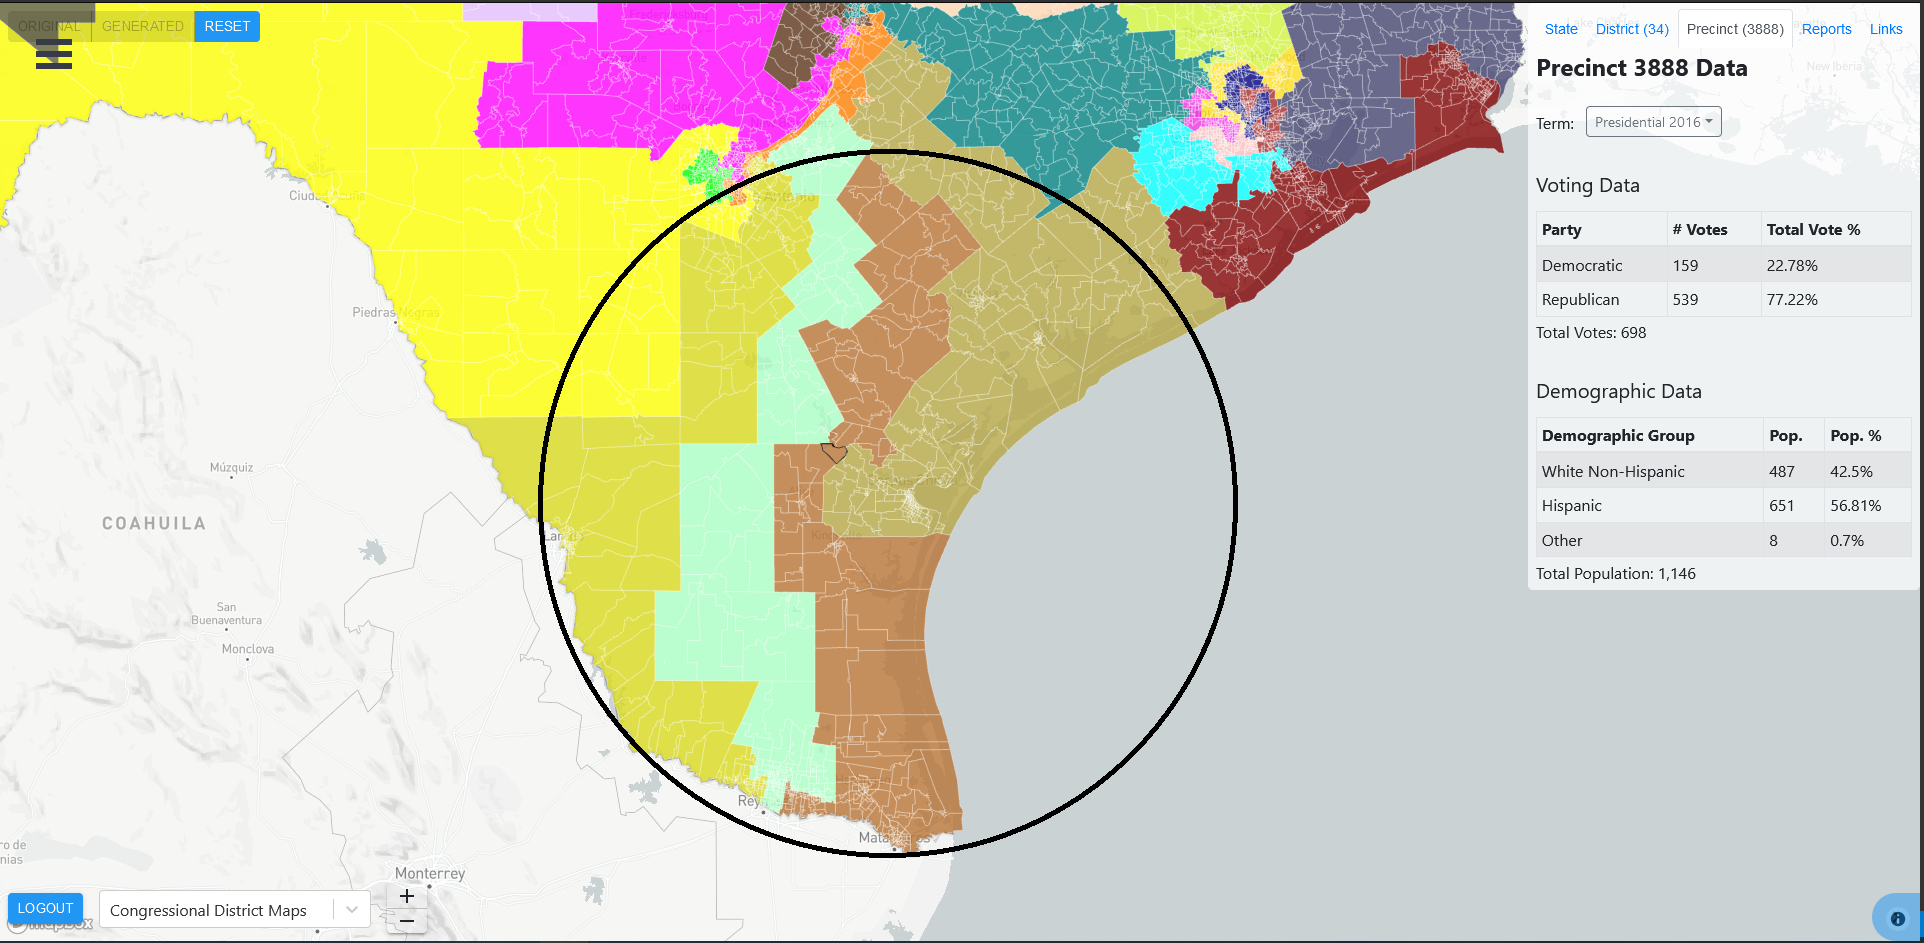
\includegraphics[width=\linewidth]{./figures/TX-34-BoundingCircle.png}
	\caption{TX-34 Bounding Circle}
	\label{fig:tx34boundingCircle}
\end{figure}

A better districting would have been to cornerize at least one of these districts, but it seems that Texas has an over-abundance of these elongated districts. In addition, not only are these districts elongated, they seem to have bottlenecks in them for the sake of lengthening the district. Specifically Precinct 3888 and Preinct 1122 which are both highlighted in the figures. The reasoning behind the lengthening is unknown but it does seem to be done with intent.

\section{Future Considerations}
With all of these case studies, there are quite a few things we can say about these measures and their strengths and weaknesses compared to human perception - which is supposed to be the ultimate judge.

Polsby-Popper is good at catching districts that have unnecessarily long boundaries by penalizing them. As a result, districts with long straight lines tend to be favored. Something that is both positive and negative is that it does not depend on what is going on outside of the district, which means that we cannot see if population groups are avoided, but on the other hand, districts are not graded based on their size as a dilation of district by any strictly positive constant still yields the same score. However, sometimes, the border looks straight from a distance but is not on closer inspection: this can give unnecessarily low scores, unless the border is smoothened, a less straightforward and undebatable process than it may appear.

The Circle Fatness measure devised, on the other hand, will “punish” long districts, and offers a solution to the issue of Polsby-Popper not taking into account what is happening right outside of the district. However, it has inherent downsides. For instance, as long as a bounding circle is small enough, the score will remain high: that is the case for OH-03 where several areas are removed from the bounding circle deeply down towards the middle, but this has a relatively limited effect on the fatness score. The opposite is true as well, the Circle Fatness is too susceptible when the district is elongated in one direction, or just covers a large area due to the population requirements.

The Convex Hull Fatness improves on the Circle Fatness' faults but it leaves things to be desired. It increases the low scores given to the elongated districts like OH-10. But there are reservations on whether this should apply to all elongated districts. Specifically, districts with a single precinct serving to create a bottleneck for the sake of elongating a district. Prominent examples discussed are TX-15 and TX-34.

% Conclusion needs to be fixed
The inherent difference between both Fatness measures and Polsby-Popper is the fact that Polsby-Popper considers only the geometric portion of fatness. Both our Circle and Convex Hull Fatness improve on this by including the population requirement that all districts in a state must be of equal population. Though these Fatness measures undoubtly fix some of Polsby-Popper's scores for some districts, it introduces questionable scores to others. Furthermore, it is to be noted that our data set was run on only nine of the fifty total states.

\printbibliography

\end{document}